\section{Generating the data set}

%TODO: Referanser til hvor vi lastet ned dataen

We have designed and implemented a method(?) to produce a realistic transit network based on the data from Mandl. The transportation time on each edge is given. The transportation demand is assumed to be known and constant. 

To do this we have constructed edges and nodes based on the data set, which consist of text files:

\begin{itemize}
\item \textbf{MandlCoords.txt} - This file includes 15 lines, with the (x,y) coordinated of the 15 nodes. These coordinated was not supplied in Mandl's literature, so these are copied from \citet{fan09} and are approximate for the picture to be drawn.

\begingroup
\obeyspaces\obeylines
\input{assets/instances/MandlCoords.txt}%
\endgroup%

\item \textbf{MandlTravelTimes.txt} - The travel times matrix gives the travel times in takes in minutes between the nodes. This matrix is symmetrical, travel times between each node and itself are zero, and ``Inf'' indicates that there is no direct link between the nodes. 

\begingroup
\obeyspaces\obeylines
\input{assets/Instances/MandlTravelTimes.txt}%
\endgroup%

\item \textbf{MandlDemand.txt} - The demand matrix shows the travel demand between each node pair, which is the average number of passenger trips per day.. This matrix is also symmetrical. (These in no demand either to or from node 15, but it is always included in the route sets because the rules that are used insist on every node being included(?)) For coding reasons, we changed the numbers in the main diagonal (from to left corner to bottom right corner) from all zero to all ’a’s. 

\begingroup
\obeyspaces\obeylines
\input{assets/Instances/MandlDemand.txt}%
\endgroup%

\end{itemize}

The nodes we create (Node.java) includes (a x,y position) their coordinates, and a number to distinguish the ants from each other. Ant(number, x, y).
The edges we create (Edge.java) includes the travel time between and the demand between two nodes. We have made edges based on the demand for each node, even though there is no direct link (travel time) between these two nodes. %TODO: skrive om hvordan vi gjør det når maurene skal velge kanter basert på travel time. 
In addition to travel time and demand, each edge includes a pheromone value to be updated after the algorithm is executed.

\begin{figure}[hb]
  \centering
  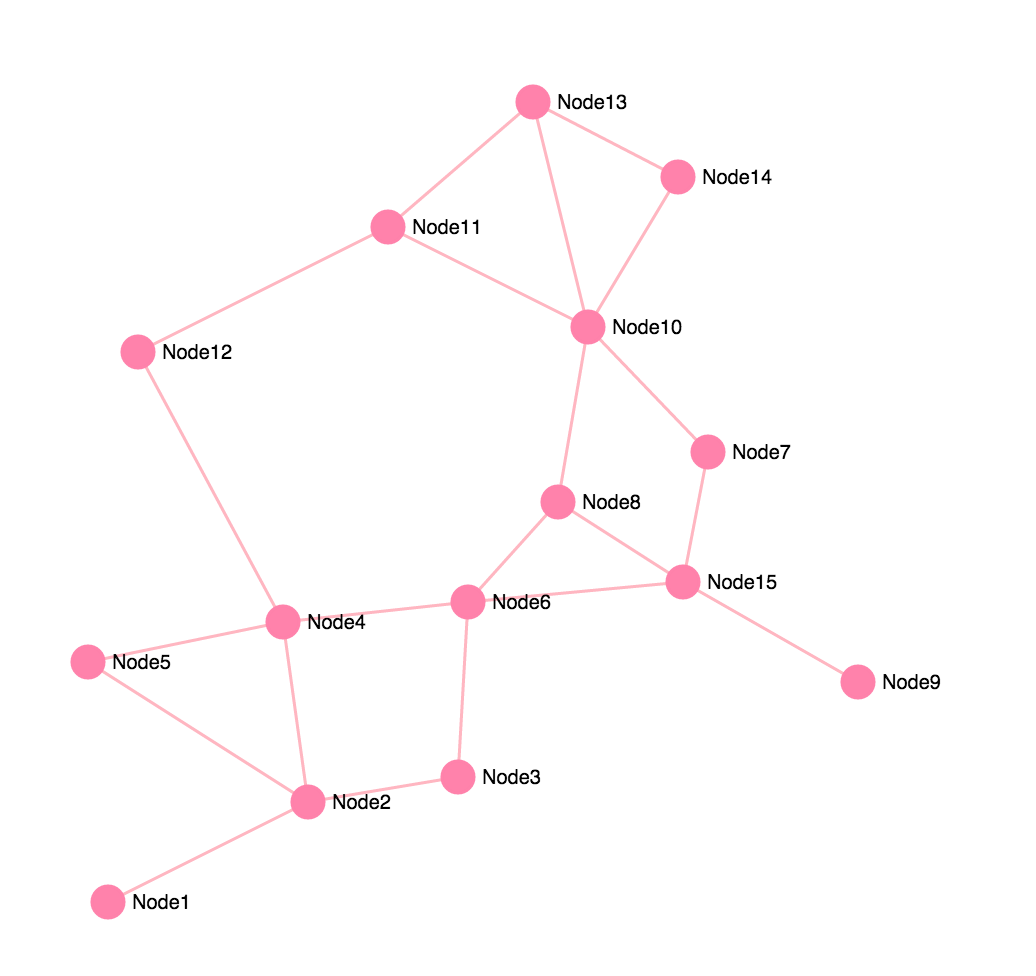
\includegraphics[width=4in]{assets/mandlnetwork.png}
  \caption[Transit Network]
   {The Transit Network, including 15 nodes and 21 edges. The graph is not directed because most lines use same arcs in both directions.}
\end{figure}
